\documentclass[useAMS,usenatbib]{mn2e}
\usepackage{footnote,graphicx,color,multirow,amsmath,url,amssymb,tabularx,amssymb}
\usepackage{hyperref}

\hypersetup{
    colorlinks,
    citecolor=blue,
    filecolor=black,
    linkcolor=black,
    urlcolor=black
}

\def\lesssim{\mathrel{\hbox{\rlap{\hbox{\lower3pt\hbox{$\sim$}}}\hbox{\raise2pt\hbox{$<$}}}}}


\begin{document}

\title[Quenching Histories of Regular and Non-Regular Rotators]{SDSS-IV MaNGA: Non-Regular Rotators Quench Faster than Regular Rotators}
\author[Smethurst et al. 2017]{R. ~J. ~Smethurst,$^{1}$ M.~Merrifield,$^{1}$ K.~L.~Masters,$^{2}$  C. ~J. ~Lintott,$^{3}$ \newauthor A.-M.~Weijmans,$^{4}$ A. Arag\'on-Salamanca,$^{1}$, N.~Drory,$^{5}$,  D.~R.~Law,$^{6}$ \newauthor J.~Brownstein,$^{7}$ K.~Bundy$^{8}$
\\ $^1$ School of Physics and Astronomy, The University of Nottingham, University Park, Nottingham, NG7 2RD, UK
\\ $^2$ Institute of Cosmology and Gravitation, University of Portsmouth, Dennis Sciama Building, Barnaby Road, Portsmouth, PO13FX, UK 
\\ $^3$ Oxford Astrophysics, Department of Physics, University of Oxford, Denys Wilkinson Building, Keble Road, Oxford, OX13RH, UK
\\ $^4$ School of Physics and Astrononomy, University of St Andrews, North Haugh, St Andrews, Fife, KY169RJ, UK
\\ $^5$ McDonald Observatory, The University of Texas at Austin, 1 University Station, Austin, TX 78712, USA
\\ $^6$ Space Telescope Science Institute, 3700 San Martin Drive, Baltimore, MD 21218, USA
\\ $^7$ Department of Physics and Astronomy, University of Utah, 115 S. 1400 E., Salt Lake City, UT 84112, USA
\\ $^8$ 	University of California, Santa Cruz, 1156 High St. Santa Cruz, CA 95064, USA
}

\maketitle

\begin{abstract}
We present a study of the star formation histories of regular and non-regular rotators. Using data from the MaNGA IFU survey, we identify a sample of non-regular rotators undergoing quenching, to which we stellar mass match a sample of quenching regular rotators, resulting in a total of $314$ galaxies. We use $u-r$ and $NUV-u$ colours from SDSS and GALEX and an existing inference package, \textsc{starpy} to conduct a pilot study of the time and exponentially declining rate that quenching has occurred in these galaxies. We find that the distribution of quenching rates across the two populations is significantly ($3.6\sigma$) different, suggesting that regular and non-regular rotators have different evolutionary histories. We find that quenching is more likely to occur at a rapid rate ($\tau \lesssim 1~\rm{Gyr}$) for non-regular rotators than across the regular rotator sample, in agreement with theories suggesting non-regular rotators are formed in dry major mergers.  We discuss how the total gas mass of a merger, rather than the merger mass ratio, may decide a galaxy's ultimate kinematic fate. 
\end{abstract}

\begin{keywords}
galaxies -- photometry, galaxies -- statistics, galaxies -- morphology
\end{keywords}

\section{Introduction}\label{sec:intro}

Recent work studying the early-type galaxy population has revealed that it is actually composed of two separate populations. The majority of early-types are rotationally supported \citep{emsellem11} with $\sim7$ times the number of regular rotators with kinematic discs (`fast' rotators), than non-regular rotators, with either dispersion dominated kinematics (`slow' rotators) or kinematically decoupled cores \citep{cappellari07, emsellem07}.  This has led to the proposal of a revision of Hubble's morphological classification scheme in the form of a `comb' \citep{cappellari16}, whereby the evolution of a galaxy, from  disc to bulge-dominated, takes place along a `tine' of the comb as a regular rotator, always retaining an underlying disc. If the discs of these regular rotators are destroyed, they then evolve along the `handle' of the comb to become non-regular rotators. 

Dry major mergers are considered the most likely process to produce non-regular rotators \citep{duc11, naab14} as they can rapidly destroy the disc dominated nature of a galaxy \citep{toomre72}. %The percentage of non-regular rotators is therefore also an estimate for the fraction of the galaxy population which have undergone a dry major merger, approximated by previous works to be $\sim10-20\%$ since $z\sim1$; \citep[][]{khochfar09}.
Regular rotators, are thought to evolve from the slow build up of a galaxy's bulge over time, eventually overwhelming the disc. This growth is thought to occur via gas-rich major or minor mergers \citep{duc11} and by gas accretion \citep{cappellari13, johnston14} which can produce a bulge dominated but rotationally supported galaxy (which would traditionally have been visually classified as an early-type in the Hubble classification scheme). %Although these mechanisms do not completely destroy the disc of a galaxy, they do cause an eventual morphological change from a pure disc to a visually bulge-dominated system.

Both major mergers and minor mergers have been postulated as quenching mechanisms \citep{hopkins08a, snyder11, hayward14}, with major mergers thought to cause a much faster quench of the remnant galaxy than a minor merger \citep{lotz08b, lotz11}. Gas accretion is also thought to cause morphological quenching; as the large gravitational potential of the bulge that builds as the accreted gas sinks to the centre of the galaxy prevents the disc from collapsing and forming stars \citep{fang13}. If regular and non-regular rotators evolve or form via these different mechanisms, we should therefore also expect to find a difference in the star formation histories of quenched regular and non-regular rotators. 

This paper documents a first look at this problem using an existing Bayesian star formation inference package, \textsc{starpy}, to determine the quenching histories of a sample of regular and non-regular rotators. We use broadband optical, $u-r$ and near-ultraviolet $NUV-u$ colours from SDSS and GALEX to infer both the time and rate that quenching has occurred in each galaxy. We aim to determine whether regular and non-regular rotating galaxies have different quenching histories. 
% before visualising the distribution of these parameters across the regular and non-regular populations. 
%This paper proceeds as follows. In Section~\ref{sec:datamethods} we describe our data sources and our Bayesian inference method for determining the quenching histories. We present our results in Section~\ref{sec:results}. We discuss the implications of our results in Section~\ref{sec:discussion}. 
The zero points of all magnitudes are in the AB system. We adopt the WMAP Seven-Year Cosmology \citep{jarosik11} with $(\Omega_m , ~\Omega_\Lambda , ~h) = (0.26, 0.73, 0.71)$.



\section{Data and Methods}\label{sec:datamethods}

\subsection{SDSS \& GALEX Photometry}\label{sec:photom}

We obtain optical photometry from the Sloan Digital Sky Survey Data Release 7 (SDSS; \citealt{york00, abazajian09}). We utilise the Petrosian magnitude, {\tt petroMag}, values for the $u$ ($3543 \rm{\AA}$) and $r$ ($6231 \rm{\AA}$) wavebands provided by the SDSS DR7 pipeline \citep{stoughton02}. Further to this, we also required NUV ($2267 \rm{\AA}$) photometry from the GALEX survey \citep{martin05}. Observed fluxes are corrected for galactic extinction \citep{Oh11} by applying the \citet*{Cardelli89} law. We also adopt $k$-corrections to $z = 0.0$ and obtain absolute magnitudes from the NYU-VAGC \citep{blanton05, padmanabhan08, blanton07}.

\subsection{MaNGA Survey \& Data Reduction Pipeline}\label{sec:manga}


MaNGA is a multi-object IFU survey conducted with the $2.5~\rm{m}$ Sloan Foundation Telescope \citep{gunn06} at Apache Point Observatory (APO) as part of SDSS-IV \citep{blanton17}. By 2020 MaNGA will have acquired IFU spectroscopy for $\sim10000$ galaxies, all with $M_* > 10^9~\rm{M}_{\odot}$ and an approximately flat mass selection (Wake et al., in preparation). The target selection does not include any cuts on morphology, colour or environment. 

In order to obtain spectra, MaNGA makes use of the Baryon Oscillation Spectroscopic Survey (BOSS) spectrograph \citep{smee13}. The BOSS spectrograph provides continuous coverage between $3600~\AA$ and $10300~\AA$ at a spectral resolution $R \sim 2000$ ($\sigma_{\rm{instrument}} \sim 77 \rm{km}~\rm{s}^{−1}$).

Complete spectral coverage to $1.5 R_e$, a galaxy's effective radius, is obtained for the majority of targets, though a subset have coverage to $2.5 R_e$. See \cite{bundy15} for an overview of the MaNGA survey. For a further description of the instrumentation used by MaNGA see \cite{drory15}. For a detailed description of the observing strategy see \cite{law15} and for  description of the survey design see \cite{yan16}. %Analysis of the prototype MaNGA (P-MaNGA) observations are presented in \cite{li15, wilkinson15, belfiore15}.

The raw data was processed by the MaNGA data reduction pipeline (DRP), which is discussed in detail \cite{law16}. The MaNGA DRP extracts, wavelength calibrates and flux calibrates all fibre spectra obtained in every exposure. The individual fibre spectra are then used to form a regular gridded datacube of $0.5''$ ‘spaxels’ and spectral channels. The spectra are logarithmically sampled with bin widths of $\log{\lambda} = 10^{-4}$. 

These datacubes are then analysed using the MaNGA data analysis pipeline (DAP); the development of which is ongoing and will be described in detail in Westfall et al. (in preparation). The primary output from the DAP are 2D ``maps" (i.e., images) of measured properties, which include flux, stellar-continuum fits, spectral index measurements and absorption- and emission-line properties. The effective radius, $R_e$, of a galaxy and the ellipticity within it, $\epsilon_e$, are provided for MaNGA galaxies in the NASA Sloan Atlas; we utilise the values measured with elliptical Petrosian apertures in {\tt v1\_0\_1} of the catalogue provided in the SDSS Data Release 13 \citep{albareti16}. 
%The DAP provides a measurement of a galaxy's effective radius, $R_e$, and the ellipticity within it, $\epsilon_e$, which is used along with the specific angular momentum to classify galaxies as either regular or non-regular rotators (see Section~\ref{sec:mangasample}). 

\subsection{Data sample}\label{sec:mangasample}

\begin{figure}
\centering
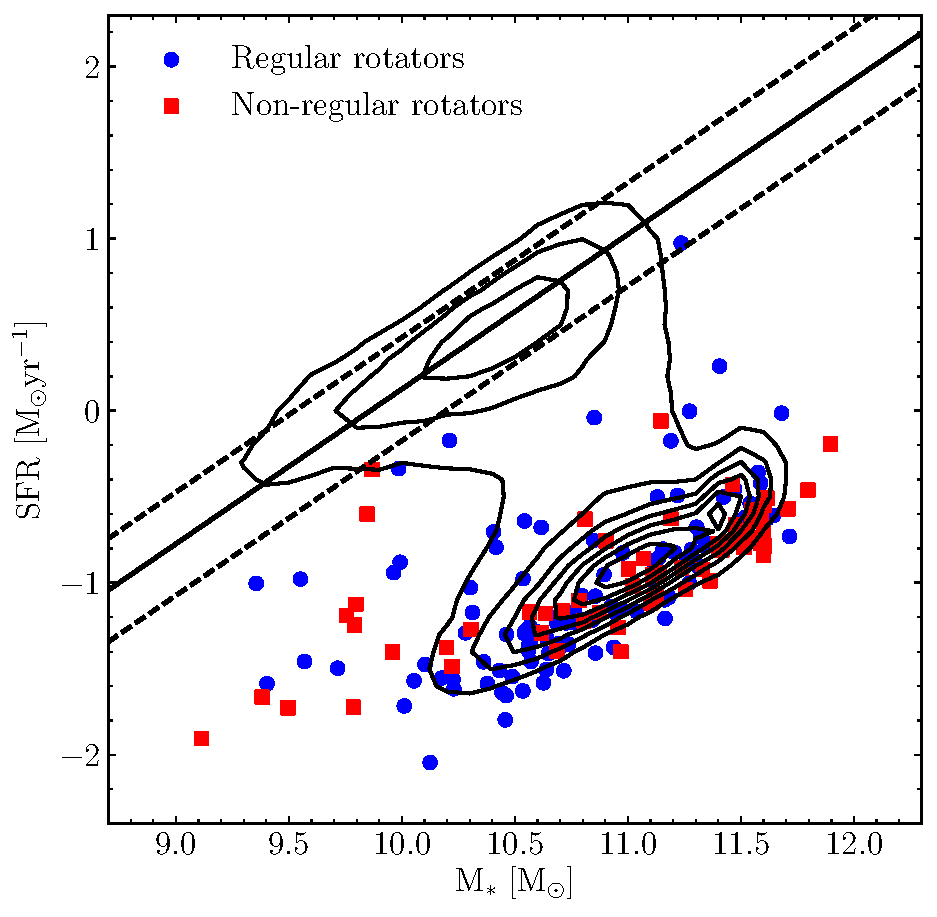
\includegraphics[width=0.475\textwidth]{../figures/nonSF_FR_SR_SFS_scatter.pdf}
\caption{Stellar mass against star formation rate for the \textsc{q-manga-galex} sample with regular (blue circles) and non-regular (red squares) rotators identified. Shown also are the contours for the entire MPA-JHU sample (black contours; i.e. SDSS DR7). The solid line shows the SFS as defined by \protect\cite{peng10} at the average redshift of the \textsc{q-manga-galex} sample with $\pm 1 \sigma$ shown by the dashed lines. Note that the galaxies in the \textsc{q-manga-galex} sample are chosen to be more than $1\sigma$ below the SFS as defined at their observed redshift and stellar mass (see Section~\protect\ref{sec:mangasample}).}
%KS Test between distributions?
\label{fig:masvsfr}
\end{figure}

There are currently $2,777$ SDSS galaxies observed by the MaNGA survey. We cross-matched these galaxies with a radius of $3''$ to the GALEX survey in order to obtain NUV photometry (see Section~\ref{sec:photom}), resulting in $1,413$ galaxies.

In this study we wish to investigate the quenching histories of these galaxies, therefore we sub-select those galaxies which are below the star forming sequence (SFS). Here we utilise the global average SFR values quoted in the MPA-JHU catalogue \citep[][which are corrected for aperture bias]{kauffmann03, brinchmann04}. We do not utilise the MaNGA spectra to calculate SFRs since the bundles only extend to $1.5~R_e$, which may result in an underestimation of the global SFR of a galaxy. 

%Whilst we do not use the MPA-JHU SFR values to infer the SFHs of these galaxies (see Section~\ref{sec:starpy}), we do utilise them to select our sample of quenching or quenched galaxies, 
We select galaxies with a SFR more than $1\sigma$ below the SFS of \cite{peng10}. Since we wish to test whether non-regular rotators quench at rapid rates, consistent with major mergers, we wish to include those galaxies which have just left the SFS (rather than selection those that are, for example, $3\sigma$ below the SFS).

This selection on SFR when applied to the \textsc{manga-galex} sample results in a sample of $838$ quenching or quenched galaxies, which we will refer to as the \textsc{q-manga-galex} sample. This sample is shown in Figure~\ref{fig:masvsfr}.

%(see Appendix section~\ref{asec:masvsfr} for a plot showing the positions of these galaxies below the SFS). 

Note that this selection will induce some bias in our sample. Regular rotators are theorised to evolve through processes which provide a fresh supply of gas for star formation, including gas-rich mergers and gas accretion. Therefore this work will only probe a specific subset of the regular rotator population. However, non-regular rotators are thought to only form through dry major mergers. If this is the case, then a non-regular rotator can only be formed from a regular rotator within which quenching is already under way. However, simulations have shown that the morphological transformation in a major merger happens before the SFR drops \cite[e.g. see][]{sparre16}. We should therefore still be able to probe whether this major merger evolution scenario exists in the non-regular rotator sample, rather than in the regular rotator sample.   

In order to classify the galaxies in the \textsc{q-manga-galex} sample as regular rotators or otherwise, we use the equation for specific stellar angular momentum as defined by \cite{emsellem07, emsellem11};
\begin{equation}
\lambda_{R_{e}} = \frac{\sum_{i=1}^{N} F_i\ R_i\ |V_i|}{\sum_{i=1}^{N} F_i\ R_i\ (V_i^2 + \sigma_i^2)^{1/2}},
\end{equation}	

where $F_i$ is the flux in the $i$th spaxel, $R_i$ the spaxel's distance from the galaxy centre (where $R_i < R_e$, the effective radius of a galaxy), $V_i$ the mean stellar velocity in that spaxel, $\sigma_i$ the stellar velocity dispersion in that spaxel and $N$ the total number of spaxels. In this work we use the python function provided in the MaNGA DAP to calculate $\lambda_{R_{e}}$ using the values of mean flux, radius, stellar velocity and stellar velocity dispersion (corrected for instrumental resolution effects) provided  by the MaNGA DAP (see Section~\ref{sec:manga}). Velocity dispersion measurements in each spaxel of a galaxy were confirmed to be above the instrument resolution of $77~\rm{km}~\rm{s}^{-1}$.

We classify galaxies in the \textsc{q-manga-galex} sample as regular or non-regular rotators using the definition from \cite{cappellari16}:
\begin{equation}
\lambda_{R_{e}} < 0.08 + \frac{\epsilon_e}{4} ~~~~~ \rm{with} ~~~~~ \epsilon_e < 0.4.
\end{equation}

Using this definition reveals $673$ ($80\%$) regular rotators and $157$ ($20\%$) non-regular rotators in the \textsc{q-manga-galex} sample. 
This is a slightly higher percentage of non-regular rotators as found by previous works \citep[$14-17\%$ of early-types; ][]{emsellem11, stott16}. Considering the fact that we do not select our sample by morphology, we would expect a smaller fraction of non-regular rotators than previous works which derived the early-type fraction of non-regular rotators. However, we believe this is offset by the fact that we also select those galaxies which lie off the SFS, a region which is typically dominated by elliptical galaxies. 

\begin{figure*}
\centering
\includegraphics[width=\textwidth]{../figures/nonSF_FR_SR_MM_sample_orig_cmap_vel_maps_large.pdf}
\caption{Ellipticity versus stellar angular momentum for the mass matched regular and non-regular rotators of the \textsc{mm-q-manga-galex} sample. Each point is shown by its stellar velocity map, each normalised to have the midpoint shown by the colour yellow. We show the separation between regular (i.e. fast) and non-regular (i.e. slow) rotators from \protect\cite{cappellari16} with the solid black line.}
%KS Test between distributions?
\label{fig:evsl}
\end{figure*}  

In order to control for the degeneracies between mass, metallicity and dust we selected a sub-sample of regular rotators matched to within $\pm~2.5~\%$ of the stellar mass of the non-regular rotators to give $157$ regular rotators. We shall refer to this sample of $314$ galaxies as the \textsc{mm-q-manga-galex} sample. An Anderson-Darling (AD) test reveals that the distribution of stellar masses of the non-regular rotators and regular rotators within this sample are statistically indistinguishable ($p=0.28$). Similarly their redshift distributions are also statistically indistinguishable ($p=0.34$).

We also consider the environmental densities of the regular and non-regular rotators by using estimates of the projected $5\rm{th}$ nearest neighbour density,  $\log\Sigma_5$, from \cite{bamford09}. An Anderson-Darling (AD) test reveals that the distribution of environment densities of the $110$ non-regular rotators and $120$ regular rotators within the \textsc{mm-q-manga-galex} sample with $\log\Sigma_5$ measurements are statistically indistinguishable ($p=0.17$). 

This is surprising since the current thinking is that non-regular rotators are more likely to be the central galaxy of a group or cluster, whereas regular rotators are more likely to be satellite galaxies \cite[see extensive review by][and references therin]{cappellari16}. Indeed, when we calculate the minimum projected separation (in degrees) of each of the galaxies in the \textsc{mm-q-manga-galex} from those of the \cite{yang09} SDSS group catalogue we find that the regular and non-regular rotators have statistically distinguishable distributions of projected separation (AD-test $p=0.005$). We find that the non-regular rotators are more likely to be the central galaxy of a group than the regular rotators of the \textsc{mm-q-manga-galex} sample. Therefore, although the projected local environment densities of the two classes of galaxies are statistically indistinguishable, their positions within that given environment density do differ, as expected. 

Given the above statistical tests, the only difference between the regular and non-regular rotators of the \textsc{mm-q-manga-galex} sample is their kinematics. This is highlighted by their velocity maps shown in Figure~\ref{fig:evsl} along with the definition of a non-regular rotator from \cite{cappellari16}, shown by the solid black line. 

%37% of the NRR are classified as ETGs (ps >=0.8) by GZ and 15% of RR. 

\subsection{SFH Inference}\label{sec:starpy}

\textsc{starpy}\footnote{Publicly available: \url{http://github.com/zooniverse/starpy}} is a \textsc{python} code which allows the inference of the exponentially declining star formation history (SFH) of a single galaxy using  Bayesian Markov Chain Monte Carlo techniques \citep{emcee13}\footnote{\url{http://dan.iel.fm/emcee/}}. The code uses the solar metallicity stellar population models of \cite[][hereafter BC03]{BC03}, assumes a Chabrier IMF \citep{chabrier03} and requires the input of the observed $u-r$ and $NUV-u$ colours and redshift. No attempt is made to model for intrinsic dust. 

The SFH is described by an exponentially declining SFR described by two parameters; the time at the onset of quenching, $t_q~\rm{[Gyr]}$, and the exponential rate at which quenching occurs, $\tau~\rm{[Gyr]}$. Under the simplifying assumption that all galaxies formed at $t=0$ $\rm{ Gyr}$ with an initial burst of star formation, the SFH can be described as:
\begin{equation}\label{sfh}
SFR =
\begin{cases}
i_{sfr}(t_q) & \text{if } t < t_q \\
i_{sfr}(t_q) \times exp{\left( \frac{-(t-t_{q})}{\tau}\right)} & \text{if } t > t_q 
\end{cases}
\end{equation}
where $i_{sfr}$ is an initial constant star formation rate dependent on $t_q$ \citep{schawinski14, smethurst15}.  A smaller $\tau$ value corresponds to a rapid quench, whereas a larger $\tau$ value corresponds to a slower quench. Note that a galaxy undergoing a slow quench is not necessarily quiescent by the time of observation. Similarly, despite a rapid quenching rate, star formation in a galaxy may still be ongoing at very low rates, rather than being fully quenched. This SFH model has previously been shown to appropriately characterise quenching galaxies \citep{Weiner06, Martin07, Noeske07,schawinski14}. 

\begin{figure*}
\centering
\includegraphics[width=\textwidth]{../figures/quenching_time_rate_FR_SR_NSF_1sigma_C16_MM.pdf}
\caption{Population densities for the time, $t_q$ (left) and exponential rate, $\tau$ (right) that quenching occurs in the \textsc{mm-q-manga-galex} sample for the regular (black, solid) and non-regular (red, dashed) rotators. A high value of $t_q$ corresponds to a recent quench, and a high value of $\tau$ corresponds to a slow quench. Shaded regions show the uncertainties on the distributions from bootstrapping. %An AD-test between the $t_q$ distributions revealed that we cannot reject ($p=0.49$) the null hypothesis that the regular and non-regular rotators quench at the same time. However, an AD-test between the $\tau$ distributions revealed that we can reject ($p=0.0003$) the hypothesis that the regular and non-regular rotators quench at the same rate. This is a $3.6\sigma$ result, suggesting that non-regular rotators quench more rapidly than regular rotators of the same mass.}
%KS Test between distributions?
}
\label{fig:popfrvsr}
\end{figure*}

We assume a flat prior on all the model parameters and model the difference between the observed and predicted $u-r$ and $NUV-u$ colours as independent realisations of a double Gaussian likelihood function (Equation 2 in \citealt{smethurst15}). We also make the simplifying assumption that the age of each galaxy, $t_\mathrm{age}$ corresponds to the age of the Universe at its observed redshift, $t_\mathrm{obs}$.

The probabilistic fitting methods to these star formation histories for an observed galaxy are described in full detail in Section 3.2 of \cite{smethurst15}, wherein the \textsc{starpy} code was used to characterise the morphologically dependence of the SFHs of $\sim126,000$ galaxies. Similarly, in \cite{smethurst16}, \textsc{starpy} was used to show the prevalence of rapid, recent quenching within a population of AGN host galaxies and in \cite{smethurst17} to investigate the quenching histories of group galaxies. An example posterior probability distribution output by \textsc{starpy} is shown for a single galaxy in Figure 5 of \cite{smethurst15}, wherein the degeneracies of the SFH model between recent, rapid quenching and earlier, slower quenching can be seen. 

To study the SFH across a sample of many galaxies, these individual posterior probability distributions are stacked in $[t_q, \tau]$ space to give a single distribution for the sample. This is no longer inference but merely a method to visualise the results for a population of galaxies (see appendix section C in \citealt{smethurst16} for a discussion on alternative methods which may be used to determine the parent population SFH). These distributions will be referred to as the population SFH densities.

\section{Results}\label{sec:results}

We determine the population SFH densities for both the regular and non-regular rotators of the \textsc{mm-q-manga-galex} sample. This is shown in Figure~\ref{fig:popfrvsr} for both the time that quenching occurs (left panel) and exponential rate of quenching (right panel) for the regular (black solid line) and non-regular (red dashed line) rotators. Uncertainties on the population densities (shown by the shaded regions) are determined from the maximum and minimum values spanned by $N = 1000$ bootstrap iterations, each sampling $90\%$ of either the regular (black shaded region) or non-regular (red shaded region) rotators. 

To statistically test the significance of our results, we estimate the `best fit' $[t_q, \tau]$ values for each galaxy with the median value of an individual galaxy's posterior probability distribution from \textsc{starpy} (i.e. the 50th percentile position of the MCMC chain). We test the distribution of these values of the regular and non-regular rotators in the \textsc{mm-q-manga-galex} sample with AD-tests. Firstly, an AD-test on the distribution of $t_q$ values for each galaxy, revealed that we cannot reject the null hypothesis that the regular and non-regular rotators quench at the same time ($AD\sim 0.3$, $p \sim 0.5$). Finally, an AD-test on the distribution of $\tau$ values for each galaxy, revealed that we can reject the null hypothesis that the fast and slow rotators quench at the same rate ($AD\sim 8.5$, $p \sim 0.0003$). This is a statistically significant ($3.6\sigma$) result, suggesting that non-regular rotators quench more rapidly than regular rotators of the same mass.


\section{Discussion}\label{sec:discussion}

The results shown in Figure~\ref{fig:popfrvsr} suggest that regular and non-regular rotators are indeed separate populations quenched, and therefore formed, by different mechanisms. However, these quenching mechanisms appear to occur at similar cosmic times for regular and non-regular rotators. Our results contradict the results of the simulations of \cite{khochfar11} who find that the last major merger interaction for slow rotators was at $z \gtrsim 1.5$ (i.e. $t_q \lesssim 4.5~\rm{Gyr}$). Contradicting the findings of \citeauthor{khochfar11}, \cite{penoyre17} find in the Illustris simulation that slow rotators only form after $z < 1$ (i.e. $t_q \gtrsim 6~\rm{Gyr}$). We note that \textsc{starpy} is not very sensitive to the time of quenching, particularly at early times i.e. $t_q \lesssim 6~\rm{Gyr}$ when $z \gtrsim 1$. Therefore, with \textsc{starpy} in its current form we cannot currently conclude which scenario our results favour. Future work altering our inference code to take spatial spectral information provided by MaNGA may help us to address this issue.

%Whilst the finding that regular rotators quench at all epochs, shown in the left panel of Figure~\ref{fig:popfrvsr}, is in agreement with previous works, for the non-regular rotators we must question whether either (i) that \textsc{starpy} is not sensitive enough to early quenching times to detect the epochs at which non-regular rotators quench (as in the \citealt{khochfar11} picture) or (ii) the degeneracies of the SFH model result in the likelihood for quenching at early times for non-regular rotators when in fact they are quenching at late times (as in the \citealt{penoyre17} picture).

We find that a fraction of the regular rotator sample quench at very slow rates ($\tau \geq 3~\rm{Gyr}$; right panel of Figure~\ref{fig:popfrvsr}). Since the \textsc{q-manga-galex} sample has not been selected by visual morphology, there will be regular rotators which are disc dominated (i.e. with bulge-to-total mass ratios of less than $0.5$ which would historically have been classified as a late-type galaxy). This likelihood for slower quenching rates is therefore likely to be caused by the effects of secular evolution through morphological quenching, slowly moving these disk galaxies off the SFS. Using the morphological classifications of Galaxy Zoo 2 \citep[GZ2][]{lintott11, GZ2} we find that $\sim 25\%$ of the regular rotators of the \textsc{mm-q-manga-galex} sample have a disk or featured debiased vote fraction, $p_d \geq 0.8$ (i.e. $80\%$ of classifiers marked the galaxy as having either a disk or features), and a debiased merger vote fraction, $p_{\rm{merger}} < 0.223$ (i.e. is not currently undergoing a merger). This is consistent (but not analogous) with the fact that $27\pm^{1}_{9}\%$ of the regular rotator quenching rate population density (black line in the right panel of Figure~\ref{fig:popfrvsr}) is found at quenching rates $\tau > 2~\rm{Gyr}$. Conversely only 4 non-regular rotators ($\sim5\%$) were classified as having a disc or features. Of these 4 galaxies $2$ have a debiased odd vote fraction, $p_{\rm{odd}} \geq 0.3$, suggesting they are undergoing either an interaction or merger. Upon visual inspection, the other $2$ galaxies are large disks with spiral structures lying outside of the MaNGA fibre bundle at $>1.5~\rm{R_e}$ and therefore outside of the $1\rm{R_e}$ radius within which $\lambda_{R_{e}}$ was calculated.

For the non-regular rotators there is very little preference for slow quenching rates with $\tau \geq 2~\rm{Gyr}$ in the right panel of Figure~\ref{fig:popfrvsr}. If we compare this with the results from \cite{smethurst15}, who found that $26.1\%$ of the quenching rate population density for  galaxies in the red sequence visually classified as `smooth' in GZ2 was at slow quenching rates (see left panel of their Figure 8). However, a `smooth' visual classification in GZ2 will include both regular and non-regular rotators. It is only in this study that we have been able to investigate the difference in the SFHs of those galaxies which are truly dispersion dominated from those which are visually early-type but which are still rotationally supported.

The prevalence of rapid rates ($\tau\lesssim1~\rm{Gyr}$) in the non-regular rotators of the \textsc{q-manga-galex} sample supports the theory that these galaxies are formed by major mergers, which are thought to cause quenching at such rates ~\citep{springel05b, bell06, lotz08b,lotz11,smethurst15}. However, we also find evidence for regular rotators quenching at these same rapid rates. Simulations have recently shown that although major mergers (2:1 or 1:1 mergers) can cause rapid quenching of a galaxy, they do not necessarily destroy the disk dominated nature of a galaxy ~\citep{pontzen16, sparre16} and can form a regular rotator \cite{bois11}. This is thought to mainly occur in gas rich major mergers \citep{bois11} and is likely the explanation for the preference for rapid rates in the regular rotator sample seen in Figure~\ref{fig:popfrvsr}. Ongoing follow up observations using the Green Bank Telescope (GBT16A-095 and GBT17A-012) to obtain HI profiles of MaNGA galaxies will help to test whether the regular rotators are indeed more gas rich than non-regular rotators in this sample. 

However \cite{bois11} also show that a gas rich major merger can produce a non-regular rotator. Upon inspection, \citeauthor{bois11} found that these tend to be those with kinematically decoupled cores, rather than the typical `slow' rotators with dispersion dominated kinematics. We have made no attempt in this study to remove galaxies with kinematically decoupled cores (or even counter rotating cores) from our non-regular rotator sample, but such a study could be the focus of future work. 

These first results studying this issue suggest that although the kinematics of regular and non-regular rotators are different in nature, the mechanisms which quench, and therefore evolve, these galaxies are very similar. However, in order to completely destroy the disk of a galaxy, some property in the formation/quenching mechanism must exceed some threshold. Since simulations have shown that it is possible for a disc to be retained in a dry major 1:1 mass ratio merger, this quantity cannot be the merger mass ratio as previously thought ~\citep{binneytremaine, bois10, tonini16}. Instead, our results showing similar quenching rates occurring across both regular and non-regular rotator samples, combined with the findings of recent simulations by ~\cite{bois11, pontzen16, sparre16}, suggest that the total gas mass fraction within a pair of merging galaxies, is what will ultimately decide the kinematic fate of a galaxy. 

\section*{Acknowledgements}

RJS gratefully acknowledges research funding from the Ogden Trust. 

Funding for the Sloan Digital Sky Survey IV has been provided by the
Alfred P. Sloan Foundation, the U.S. Department of Energy Office of
Science, and the Participating Institutions. SDSS acknowledges
support and resources from the Center for High-Performance Computing at the University of Utah. The SDSS web site is \url{www.sdss.org}.

SDSS is managed by the Astrophysical Research Consortium for the Participating Institutions of the SDSS Collaboration including the Brazilian Participation Group, the Carnegie Institution for Science, Carnegie Mellon University, the Chilean Participation Group, the French Participation Group, Harvard-Smithsonian Center for Astrophysics, Instituto de Astrof\'isica de Canarias, The Johns Hopkins University, Kavli Institute for the Physics and Mathematics of the Universe (IPMU) / University of Tokyo, Lawrence Berkeley National Laboratory, Leibniz Institut für Astrophysik Potsdam (AIP), Max-Planck-Institut f\"ur Astronomie (MPIA Heidelberg), Max-Planck-Institut für Astrophysik (MPA Garching), Max-Planck-Institut f\"ur Extraterrestrische Physik (MPE), National Astronomical Observatories of China, New Mexico State University, New York University, University of Notre Dame, Observat\'orio Nacional / MCTI, The Ohio State University, Pennsylvania State University, Shanghai Astronomical Observatory, United Kingdom Participation Group, Universidad Nacional Aut\'onoma de M\'exico, University of Arizona, University of Colorado Boulder, University of Oxford, University of Portsmouth, University of Utah, University of Virginia, University of Washington, University of Wisconsin, Vanderbilt University and Yale University.

\bibliographystyle{mn2e}
\bibliography{refs}  

% \appendix

% \section{Location of galaxies on SFS}\label{asec:masvsfr}

% Figure~\ref{fig:masvsfr} shows the location of the non-regular and mass matched regular rotators of the \textsc{mm-q-manga-galex} lying more than $1\sigma$ below the SFS.



\end{document}
